\chapter{Toroidal Coordinate System}
The flux surface geometry of the standard magnetic configuration of the Wendelstein 7-X~(\mbox{W7-X}) stellarator is shown in Fig.~\ref{fig:w7x_ref_1}
as an example for the type of geometry discussed for in this chapter.
\begin{figure}[htbp]
  \centering
  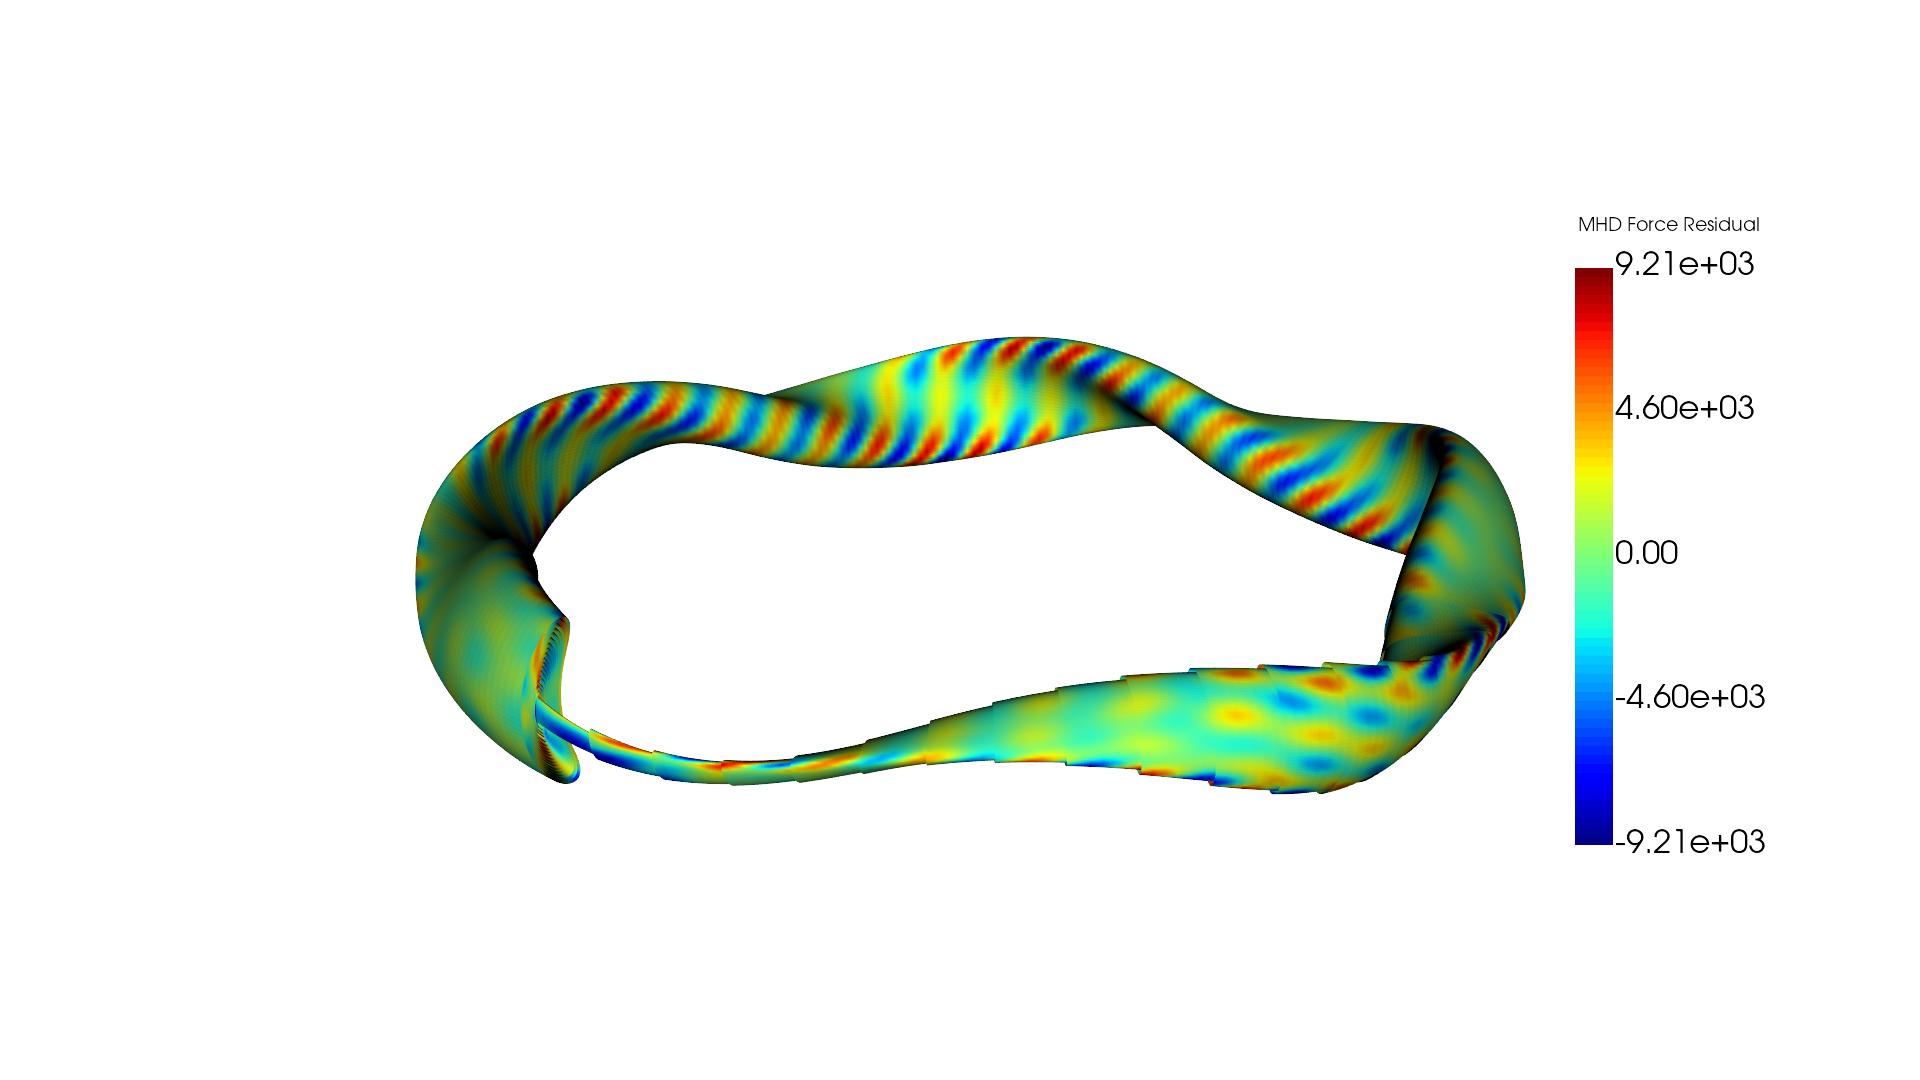
\includegraphics[width=0.9\textwidth]{img/vmecpp_w7x_1921.png}
  \caption{Flux surface geometry and MHD force residual color-coded on it,
           of the standard magnetic configuration of the Wendelstein 7-X stellarator.
           Some of the flux surface are shown as cut-open to see the inner surfaces.}
  \label{fig:w7x_ref_1}
\end{figure}
%
\FloatBarrier
In Fig.~\ref{fig:torcoords}, the toroidal coordinate system in use is shown.
\begin{figure}[htbp]
  \centering
  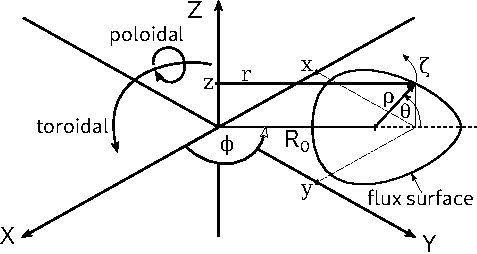
\includegraphics[width=0.7\textwidth]{img/toroidal_coordinates.pdf}
  \caption{Coordinate systems in use in this work.
           A poloidal cut through a flux surface at the toroidal angle $\phi$ is shown.
           A point on the (torus-like) flux surface can be uniquely specified
           either by its Cartesian coordinates $(x,y,z)$,
           by its cylindrical coordinates $(r, \phi, z)$ or
           by its toroidal coordinates $(\rho,\theta,\phi)$.
           $R_0$ is the major radius of the toroidal coordinate system at $\phi$.}
  \label{fig:torcoords}
\end{figure}
%
Note that a point on a flux surface is described uniquely by three sets of coordinates:
$(x,y,z)$ in Cartesian coordinates, $(r, \phi, z)$ in cylindrical coordinates and $(\rho, \theta, \phi)$ in toroidal coordinates.
All three coordinate systems are orthogonal. The Cartesian and the cylindrical coordinate systems are right-handed
and the choice of the poloidal angle as illustrated implies that the toroidal coordinate system is left-handed.

\FloatBarrier
\section{Inverse Coordinate Representation}
A toroidal surface like this is conveniently parameterized by two angle-like coordinates.
The long way around the torus (along its major circumference) is called the toroidal direction
and the short way around the torus (wristband-like) is called the poloidal direction (cf Fig.~\ref{fig:torcoords}).
The toroidal coordinate is $\zeta$ and the poloidal coordinate is $\theta$.
This torus is embedded in a cylindrical coordinate system,
where the $z$-axis is aligned with the major axis of the torus.
The cylindrical angle $\phi$ can be identified with the toroidal coordinate~$\zeta$ of the torus,
although usually one introduces an integer scaling factor to exploit toroidal symmetry (see below).
Note that this works only for singly-linked tori, whereas knotted configurations need a special treatment~\cite{hudson_knotatrons}.
This allows to specify the surface geometry using two-dimensional discrete Fourier series in $\theta$ and $\zeta$
for the coordinates $R$ and $Z$ of a surface:
\begin{align}
  R(\theta, \zeta) =&\, \realpart \left( \sum_{m=-\infty}^{+\infty} \sum_{n=-\infty}^{+\infty} \hat{R}_{m,n} \,e^{-i (m \theta + n \zeta)} \right) \nonumber \\
  Z(\theta, \zeta) =&\, \realpart \left( \sum_{m=-\infty}^{+\infty} \sum_{n=-\infty}^{+\infty} \hat{Z}_{m,n} \,e^{-i (m \theta + n \zeta)} \right) \nonumber
\end{align}
where $\theta$ is the poloidal angle-like coordinate, $m$ and $n$ are (integer) poloidal and toroidal mode numbers, respectively,
and $\hat{R}_{m,n}$, $\hat{Z}_{m,n}$ are the (complex-valued) Fourier coefficients of $R$ and $Z$, respectively.
In VMEC, the toroidal coordinates $(\rho, \theta, \zeta)$ form a left-handed coordinate system
due to the chosen direction for the poloidal coordinate $\theta$ depicted in Fig.~\ref{fig:torcoords}.
The sign of $\theta$ is therefore inverted in the Fourier representation:
\begin{align}
  R(\theta, \zeta) =&\, \realpart \left( \sum_{m=-\infty}^{+\infty} \sum_{n=-\infty}^{+\infty} \hat{R}_{m,n} \,e^{-i (m (-\theta) + n \zeta)} \right)
                   =    \realpart \left( \sum_{m=-\infty}^{+\infty} \sum_{n=-\infty}^{+\infty} \hat{R}_{m,n} \,e^{ i (m   \theta  - n \zeta)} \right) \label{eqn:R} \\
  Z(\theta, \zeta) =&\, \realpart \left( \sum_{m=-\infty}^{+\infty} \sum_{n=-\infty}^{+\infty} \hat{Z}_{m,n} \,e^{-i (m (-\theta) + n \zeta)} \right)
                   =    \realpart \left( \sum_{m=-\infty}^{+\infty} \sum_{n=-\infty}^{+\infty} \hat{Z}_{m,n} \,e^{ i (m   \theta  - n \zeta)} \right) \label{eqn:Z} \, .
\end{align}
Note that the specification of the surface geometry in \eqn{R} and \eqn{Z} is somewhat inconvenient to implement numerically:
it needs complex arithmetics and it features infinite sums over the mode numbers.
These issues are dealt with by two simplicifications outlined in the following.
First, the complex Fourier coefficients and complex basis functions are split into real and imaginary parts and rearranged.
This is illustrated exemplarly for $R$:
\begin{align}
  R(\theta, \zeta) =&\, \realpart \left( \sum_{m=-\infty}^{+\infty} \sum_{n=-\infty}^{+\infty}
                       \hat{R}_{m,n} \,e^{ i (m   \theta  - n \zeta)} \right)        \nonumber                 \\
                   =&\, \realpart \left( \sum_{m=-\infty}^{+\infty} \sum_{n=-\infty}^{+\infty}
                       \left( \hat{R}_{m,n}^\mathrm{Re} + i \cdot \hat{R}_{m,n}^\mathrm{Im} \right) \cdot
                       \left(  \cos(m \theta  - n \zeta) + i \cdot  \sin(m \theta  - n \zeta) \right) \right) \label{eqn:cplxR}
\end{align}
with $\hat{R}_{m,n}^\mathrm{Re} = \realpart \left( \hat{R}_{m,n} \right)$
and  $\hat{R}_{m,n}^\mathrm{Im} = \imagpart \left( \hat{R}_{m,n} \right)$.
Now consider the complex multiplication in \eqn{cplxR} separately:
\begin{align}
  ~& \left( \hat{R}_{m,n}^\mathrm{Re} + i \cdot \hat{R}_{m,n}^\mathrm{Im} \right) \cdot
     \left(  \cos(m \theta  - n \zeta) + i \cdot  \sin(m \theta  - n \zeta) \right) \nonumber \\
  =& \phantom{+ i \cdot}~~ \left( \hat{R}_{m,n}^\mathrm{Re} \cos(m \theta - n \zeta) - \hat{R}_{m,n}^\mathrm{Im} \sin(m \theta - n \zeta) \right) \nonumber \\
  ~&          + i \cdot    \left( \hat{R}_{m,n}^\mathrm{Re} \sin(m \theta - n \zeta) + \hat{R}_{m,n}^\mathrm{Im} \cos(m \theta - n \zeta) \right)
\end{align}
Only the real part of above result is required to express $R$ and the imaginary part is ignored.
The Fourier coefficients for $R$ are renamed after their (now real-valued) Fourier basis functions:
\begin{align}
  \hat{R}_{m,n}^\mathrm{cos} \equiv& \phantom{-}~ \hat{R}_{m,n}^\mathrm{Re} \\
  \hat{R}_{m,n}^\mathrm{sin} \equiv&          -   \hat{R}_{m,n}^\mathrm{Im}
\end{align}
and equivalently for $Z$:
\begin{align}
  \hat{Z}_{m,n}^\mathrm{cos} \equiv& \phantom{-}~ \hat{Z}_{m,n}^\mathrm{Re} \\
  \hat{Z}_{m,n}^\mathrm{sin} \equiv&          -   \hat{Z}_{m,n}^\mathrm{Im} \, .
\end{align}
This results in the following representation, which only involves real arithmetics now:
\begin{align}
  R(\theta, \zeta) =& \sum_{m=-\infty}^{+\infty} \sum_{n=-\infty}^{+\infty} \left( \hat{R}_{m,n}^\mathrm{cos} \cos(m \theta - n \zeta) + \hat{R}_{m,n}^\mathrm{sin} \sin(m \theta - n \zeta) \right) \nonumber \\
  Z(\theta, \zeta) =& \sum_{m=-\infty}^{+\infty} \sum_{n=-\infty}^{+\infty} \left( \hat{Z}_{m,n}^\mathrm{cos} \cos(m \theta - n \zeta) + \hat{Z}_{m,n}^\mathrm{sin} \sin(m \theta - n \zeta) \right) \nonumber \, .
\end{align}
Second, the Fourier spectrum of $R$ and $Z$ is truncated at some finite maximim mode numbers $M$ and $N$:
\begin{align}
  R(\theta, \zeta) =& \sum_{m=-M}^{M} \sum_{n=-N}^{N}
                       \left( \hat{R}_{m,n}^\mathrm{cos} \cos(m \theta - n \zeta) + \hat{R}_{m,n}^\mathrm{sin} \sin(m \theta - n \zeta) \right) \label{eqn:R2} \\
  Z(\theta, \zeta) =& \sum_{m=-M}^{M} \sum_{n=-N}^{N}
                       \left( \hat{Z}_{m,n}^\mathrm{cos} \cos(m \theta - n \zeta) + \hat{Z}_{m,n}^\mathrm{sin} \sin(m \theta - n \zeta) \right) \label{eqn:Z2} \, .
\end{align}
A sketch of the layout of the full mode spectrum used in \eqn{R2} and \eqn{Z2} is shown in Fig.~\ref{fig:mode_numbers}.
\begin{figure}[htbp]
  \centering
  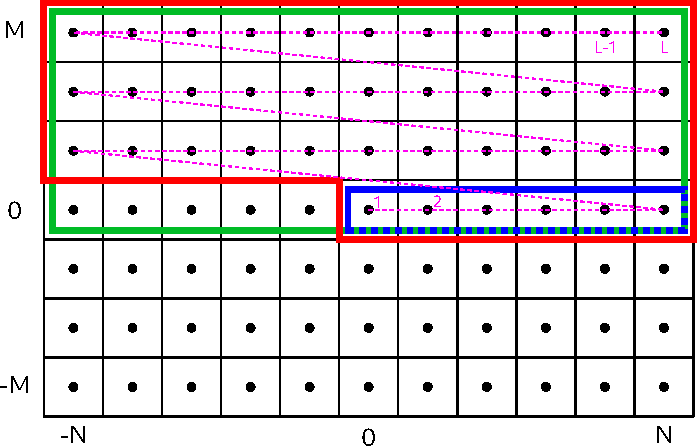
\includegraphics{img/mode_numbers.pdf}
  \caption{Full mode number spectrum used in \eqn{R2} and \eqn{Z2} (black grid)
           for $M=3$ and $N=5$.
           The horizontal axis enumerates toroidal mode numbers $-N \leq n \leq N$
           and the vertical axis enumerated poloidal mode numbers $-M \leq m \leq M$.
           Single Fourier modes are represented by black dots in the grid cells.
           %The dashed lines at $m=0$ and $n=0$ shall guide the eye.
           The green rectangle contains the modes with $m \geq 0$.
           The blue rectangle contains the modes with $m=0$ and $n \geq 0$.
           The red polygon includes all mode number combinations required to uniquely define a real-space quantity, e.g., $R$ or $Z$.
           The pink dashed line and the pink numbers indicate the linear arrangement of the Fourier harmonics
           used to vectorize the numerical implementation.}
  \label{fig:mode_numbers}
\end{figure}
Redundant information among the Fourier harmonics $\hat{R}_{m,n}$ and $\hat{Z}_{m,n}$ is eliminated
by taking into account only modes with $0 \leq m \leq M$ and $|n| \leq N$,
which still fully define the (truncated) Fourier representation, as is shown in the following.
For any $(\theta, \zeta) \in \realnumbers$ and given mode numbers $(m,n)$ with $m < 0$ it holds:
\begin{align}
    \cos(m \theta - n \zeta)
 =& \cos\left(- ( m  \theta -   n  \zeta)\right) \nonumber \\
 =& \cos\left(  (-m) \theta - (-n) \zeta \right) \nonumber \\
 =& \cos\left(  m' \theta - n' \zeta \right)
\end{align}
and similarly:
\begin{align}
      \sin(m \theta - n \zeta)
 =& - \sin\left(- ( m  \theta -   n  \zeta)\right) \nonumber \\
 =& - \sin\left(  (-m) \theta - (-n) \zeta \right) \nonumber \\
 =& - \sin\left(  m' \theta - n' \zeta \right)
\end{align}
with $m' = -m$ and $n' = -n$ where now $m' > 0$.
Thus, the Fourier coefficients for $m<0$ can either be included in the Fourier series for $R$ and $Z$
by weighting them with their own basis functions
or they can equivalently be included in the Fourier coefficients for $m>0$ as follows:
\begin{align}
 \tilde{R}_{m,n}^\mathrm{cos} =& \hat{R}_{m,n}^\mathrm{cos} + \hat{R}_{-m,-n}^\mathrm{cos} \\
 \tilde{R}_{m,n}^\mathrm{sin} =& \hat{R}_{m,n}^\mathrm{sin} - \hat{R}_{-m,-n}^\mathrm{sin}
\end{align}
and analogously for $Z$:
\begin{align}
 \tilde{Z}_{m,n}^\mathrm{cos} =& \hat{Z}_{m,n}^\mathrm{cos} + \hat{Z}_{-m,-n}^\mathrm{cos} \\
 \tilde{Z}_{m,n}^\mathrm{sin} =& \hat{Z}_{m,n}^\mathrm{sin} - \hat{Z}_{-m,-n}^\mathrm{sin}
\end{align}
for $0 \leq m \leq M$ and $-N \leq n \leq N$.
Using these combined Fourier coefficients
    $\tilde{R}_{m,n}^\mathrm{cos}$, $\tilde{R}_{m,n}^\mathrm{sin}$
and $\tilde{Z}_{m,n}^\mathrm{cos}$, $\tilde{Z}_{m,n}^\mathrm{sin}$,
the number of summands in \eqn{R2} and \eqn{Z2} can already be almost halved:
\begin{align}
  R(\theta, \zeta) =& \sum_{m=0}^{M} \sum_{n=-N}^{N}
                       \left( \tilde{R}_{m,n}^\mathrm{cos} \cos(m \theta - n \zeta) + \tilde{R}_{m,n}^\mathrm{sin} \sin(m \theta - n \zeta) \right) \nonumber \\
  Z(\theta, \zeta) =& \sum_{m=0}^{M} \sum_{n=-N}^{N}
                       \left( \tilde{Z}_{m,n}^\mathrm{cos} \cos(m \theta - n \zeta) + \tilde{Z}_{m,n}^\mathrm{sin} \sin(m \theta - n \zeta) \right) \nonumber
\end{align}
which is equivalent to the green rectangle in Fig.~\ref{fig:mode_numbers}.
One further possible way of compression becomes evident when considering the Fourier basis for $m=0$.
Note that:
\begin{align}
 \cos(\underbrace{m \theta}_{=0} -n \zeta) =& \phantom{-}~ \cos(n \zeta) \label{eqn:m0cos} \\
 \sin(\underbrace{m \theta}_{=0} -n \zeta) =&          -   \sin(n \zeta) \label{eqn:m0sin} \, .
\end{align}
Thus, the Fourier coefficients for $m=0$ and $n<0$ can be combined with the ones for $m=0$ and $n>0$ as follows:
\begin{align}
 \tilde{\tilde{R}}_{0,n}^\mathrm{cos} \equiv& \phantom{-}~ \tilde{R}_{0,n}^\mathrm{cos} + \tilde{R}_{0,-n}^\mathrm{cos} \\
 \tilde{\tilde{R}}_{0,n}^\mathrm{sin} \equiv&          -   \tilde{R}_{0,n}^\mathrm{sin} + \tilde{R}_{0,-n}^\mathrm{sin}
\end{align}
where yet another sign change was performed for $\tilde{\tilde{R}}_{0,n}^\mathrm{sin}$ to cancel
the minus in the right-hand side of \eqn{m0sin}.
Analogous expressions follow for $Z$:
\begin{align}
 \tilde{\tilde{Z}}_{0,n}^\mathrm{cos} \equiv& \phantom{-}~ \tilde{Z}_{0,n}^\mathrm{cos} + \tilde{Z}_{0,-n}^\mathrm{cos} \\
 \tilde{\tilde{Z}}_{0,n}^\mathrm{sin} \equiv&          -   \tilde{Z}_{0,n}^\mathrm{sin} + \tilde{Z}_{0,-n}^\mathrm{sin} \, .
\end{align}
In the end, the two-dimensional Fourier series for $R$ and $Z$ can be written as follows:
\begin{align}
    R(\theta, \zeta)
 =& \phantom{+ \sum_{m=1}^{M}}~~\, \sum_{n=0}^{N}
      \left( \tilde{\tilde{R}}_{0,n}^\mathrm{cos} \cos(n \zeta) + \tilde{\tilde{R}}_{0,n}^\mathrm{sin} \sin(n \zeta) \right) \nonumber \\
 ~&          + \sum_{m=1}^{M}   \sum_{n=-N}^{N}
      \left( \tilde{R}_{m,n}^\mathrm{cos} \cos(m \theta - n \zeta) + \tilde{R}_{m,n}^\mathrm{sin} \sin(m \theta - n \zeta) \right) \nonumber \\
 =& \phantom{+}\, \sum_{n=0}^{N}                 \tilde{\tilde{R}}_{0,n}^\mathrm{cos} \cos(n \zeta)
             +    \sum_{m=1}^{M} \sum_{n=-N}^{N} \tilde{R}_{m,n}^\mathrm{cos}         \cos(m \theta - n \zeta) \nonumber \\
 ~&          +    \sum_{n=1}^{N}                 \tilde{\tilde{R}}_{0,n}^\mathrm{sin} \sin(n \zeta)
             +    \sum_{m=1}^{M} \sum_{n=-N}^{N} \tilde{R}_{m,n}^\mathrm{sin}         \sin(m \theta - n \zeta) \label{eqn:fullFourierR} \\
    Z(\theta, \zeta)
 =& \phantom{+ \sum_{m=1}^{M}}~~\, \sum_{n=0}^{N}
      \left( \tilde{\tilde{Z}}_{0,n}^\mathrm{cos} \cos(n \zeta) + \tilde{\tilde{Z}}_{0,n}^\mathrm{sin} \sin(n \zeta) \right) \nonumber \\
 ~&          + \sum_{m=1}^{M}   \sum_{n=-N}^{N}
      \left( \tilde{Z}_{m,n}^\mathrm{cos} \cos(m \theta - n \zeta) + \tilde{Z}_{m,n}^\mathrm{sin} \sin(m \theta - n \zeta) \right) \nonumber \\
 =& \phantom{+}\, \sum_{n=0}^{N}                 \tilde{\tilde{Z}}_{0,n}^\mathrm{cos} \cos(n \zeta)
             +    \sum_{m=1}^{M} \sum_{n=-N}^{N} \tilde{Z}_{m,n}^\mathrm{cos}         \cos(m \theta - n \zeta) \nonumber \\
 ~&          +    \sum_{n=1}^{N}                 \tilde{\tilde{Z}}_{0,n}^\mathrm{sin} \sin(n \zeta)
             +    \sum_{m=1}^{M} \sum_{n=-N}^{N} \tilde{Z}_{m,n}^\mathrm{sin}         \sin(m \theta - n \zeta) \label{eqn:fullFourierZ} \, .
\end{align}
Note that the $(0,0)$-Fourier coefficients for sine basis functions are redundant,
since $\sin(0\, \theta + 0\, \zeta) = 0$ for all values of $\theta$ and $\zeta$.
Thus, no matter what the value of $\tilde{\tilde{R}}_{0,0}^\mathrm{sin}$ or $\tilde{\tilde{Z}}_{0,0}^\mathrm{sin}$ would be,
their contributions would not enter into $R$ or $Z$, respectively, anyway.

\FloatBarrier
\newpage
\section{Symmetry Properties}
The surface geometry depicted in Fig.~\ref{fig:w7x_ref_1} features a five-fold symmetry in the toroidal direction
which can be taken into account to further reduce the number of Fourier coefficients required to describe the surface geometry.
The toroidal periodicity of the surface is denoted $n_\mathrm{fp}$ ($=5$ for W7-X).
Note that for a (axisymmetric) Tokamak, $n_\mathrm{fp}=1$ and $N=0$ are sufficient to describe the toroidal direction.
The cylindrical angle $\phi$ is now brought into correspondence with the toroidal coordinate $\zeta$
by the following relation:
\begin{equation}
  \zeta = n_\mathrm{fp} \cdot \phi \label{eqn:zeta} \, .
\end{equation}
Frequently, the Fourier representation of the surface geometry is written in terms as $\phi$ instead of $\zeta$:
\begin{align}
    R(\theta, \phi)
 =& \phantom{+ \sum_{m=1}^{M}}~~\, \sum_{n=0}^{N}
      \left( \tilde{\tilde{R}}_{0,n}^\mathrm{cos} \cos(n n_\mathrm{fp} \phi) + \tilde{\tilde{R}}_{0,n}^\mathrm{sin} \sin(n n_\mathrm{fp} \phi) \right) \nonumber \\
 ~&          + \sum_{m=1}^{M}   \sum_{n=-N}^{N}
      \left( \tilde{R}_{m,n}^\mathrm{cos} \cos(m \theta - n n_\mathrm{fp} \phi) + \tilde{R}_{m,n}^\mathrm{sin} \sin(m \theta - n n_\mathrm{fp} \phi) \right) \label{eqn:fullFourierRPhi} \\
    Z(\theta, \phi)
 =& \phantom{+ \sum_{m=1}^{M}}~~\, \sum_{n=0}^{N}
      \left( \tilde{\tilde{Z}}_{0,n}^\mathrm{cos} \cos(n n_\mathrm{fp} \phi) + \tilde{\tilde{Z}}_{0,n}^\mathrm{sin} \sin(n n_\mathrm{fp} \phi) \right) \nonumber \\
 ~&          + \sum_{m=1}^{M}   \sum_{n=-N}^{N}
      \left( \tilde{Z}_{m,n}^\mathrm{cos} \cos(m \theta - n n_\mathrm{fp} \phi) + \tilde{Z}_{m,n}^\mathrm{sin} \sin(m \theta - n n_\mathrm{fp} \phi) \right) \label{eqn:fullFourierZPhi} \, .
\end{align}
The $\zeta$ coordinate is also called toroidal angle per module,
since it advances by $2 \pi$ when going from one toroidal module to the next one.
Toroidal symmetry is expressed in mathematical form as follows:
\begin{align}
  R(\theta, \zeta) =& R \left( \theta, \zeta + 2 \pi k \right) \\
  Z(\theta, \zeta) =& Z \left( \theta, \zeta + 2 \pi k \right)
\end{align}
and equivalently for $\phi$:
\begin{align}
  R(\theta, \phi) =& R \left( \theta, \phi + \frac{2 \pi k}{n_\mathrm{fp}} \right) \\
  Z(\theta, \phi) =& Z \left( \theta, \phi + \frac{2 \pi k}{n_\mathrm{fp}} \right)
\end{align}
for $k \in \integers$.
Note that while $\phi$ takes on values between $0$ and $2 \pi$ for a full toroidal turn,
the $\zeta$-coordinates takes on values between $0$ and $n_\mathrm{fp} \cdot (2 \pi)$ for a full toroidal turn
around the whole machine.

One further symmetry property, commonly referred to as stellarator symmetry,
can be taken into account (if applicable) to reduce the number of Fourier coefficients.
It is observed that each of the $n_\mathrm{fp}$ toroidal modules is flip-symmetric about the axis in the $(x,y)$-plane at half its toroidal angle
as well as the axis in the $(x,y)$-plane at its toroidal boundaries.
This symmetry property is expressed as follows:
\begin{align}
  R(\theta, \zeta) =& \phantom{-}~ R(-\theta, -\zeta) \\
  Z(\theta, \zeta) =&          -   Z(-\theta, -\zeta) \, .
\end{align}
In order to recover this symmetry property in the Fourier representation of $R$ and $Z$,
it is required to only take into account Fourier coefficients for $R$ and $Z$ with appropriate parity.
For $R$, which needs to retain even parity, these are all Fourier coefficients weighted by cosine basis functions.
For $Z$, which needs to retain  odd parity, these are all Fourier coefficients weighted by sine basis functions.
Therefore, a stellarator-symmetric surface can be expressed as follows:
\begin{align}
    R(\theta, \zeta)
 =&                  \sum_{n= 0}^{N} \tilde{\tilde{R}}_{0,n}^\mathrm{cos}            \cos(n \zeta)
    + \sum_{m=1}^{M} \sum_{n=-N}^{N}         \tilde{R}_{m,n}^\mathrm{cos} \cos(m \theta - n \zeta) \label{eqn:stellsymR} \\
    Z(\theta, \zeta)
 =&                  \sum_{n= 0}^{N} \tilde{\tilde{Z}}_{0,n}^\mathrm{sin}            \sin(n \zeta)
    + \sum_{m=1}^{M} \sum_{n=-N}^{N}         \tilde{Z}_{m,n}^\mathrm{sin} \sin(m \theta - n \zeta) \label{eqn:stellsymZ}
\end{align}
and similarly for $\phi$:
\begin{align}
    R(\theta, \phi)
 =&                  \sum_{n= 0}^{N} \tilde{\tilde{R}}_{0,n}^\mathrm{cos}            \cos(n n_\mathrm{fp} \phi)
    + \sum_{m=1}^{M} \sum_{n=-N}^{N}         \tilde{R}_{m,n}^\mathrm{cos} \cos(m \theta - n n_\mathrm{fp} \phi) \label{eqn:stellsymRPhi} \\
    Z(\theta, \phi)
 =&                  \sum_{n= 0}^{N} \tilde{\tilde{Z}}_{0,n}^\mathrm{sin}            \sin(n n_\mathrm{fp} \phi)
    + \sum_{m=1}^{M} \sum_{n=-N}^{N}         \tilde{Z}_{m,n}^\mathrm{sin} \sin(m \theta - n n_\mathrm{fp} \phi) \label{eqn:stellsymZPhi} \, .
\end{align}
The terms only required when no stellarator symmetry can be assumed are marked {\color{blue}blue} from here on.

\FloatBarrier
\section{Vectorized Formulation of Fourier Series} \label{sec:torcoords_numbering}
It is evident that the Fourier summation for $R$ and $Z$ in \eqn{fullFourierRPhi} and \eqn{fullFourierZPhi}
and also for the stellarator-symmetric case in \eqn{stellsymRPhi} and \eqn{stellsymZPhi}
is rather complicated in terms of which coefficients to take into account and which not.
Efficiently implementing these expressions numerically would be rather difficult.
In order to fix this, the Fourier coefficients are arranged along one linear dimension
and appropriate mode number arrays are introduced.
The total number of mode number combinations to take into account is:
\begin{equation}
 K = (N + 1) + M (2N + 1) \, .
\end{equation}
The order in which the mode numbers and the Fourier coefficients appear in the linear arragement is shown in Tab.~\ref{tab:xm_xn_contents}.
\begin{table}[htb]
  \centering
  \begin{tabular}{c|c|c|c|c|c|c}
    index $k$ & $m_k \equiv m$ & $n_k \equiv n_\mathrm{fp} n$ &               $R_k^\mathrm{cos}$       &               $Z_k^\mathrm{sin}$       & {\color{blue}               $R_k^\mathrm{sin}$       } & {\color{blue}               $Z_k^\mathrm{cos}$       } \\
    \hline %  &                &                              &                                        &                                        & {\color{blue}                                        } & {\color{blue}                                        } \\
    1         & 0              & 0                            & $\tilde{\tilde{R}}_{0,0}^\mathrm{cos}$ & $\tilde{\tilde{Z}}_{0,0}^\mathrm{sin}$ & {\color{blue} $\tilde{\tilde{R}}_{0,0}^\mathrm{sin}$ } & {\color{blue} $\tilde{\tilde{Z}}_{0,0}^\mathrm{cos}$ } \\
    ...       & 0              & ...                          & ...                                    & ...                                    & {\color{blue} ...                                    } & {\color{blue} ...                                    } \\
    $N+1$     & 0              & $  n_\mathrm{fp} N$          & $\tilde{\tilde{R}}_{0,N}^\mathrm{cos}$ & $\tilde{\tilde{Z}}_{0,N}^\mathrm{sin}$ & {\color{blue} $\tilde{\tilde{R}}_{0,N}^\mathrm{sin}$ } & {\color{blue} $\tilde{\tilde{Z}}_{0,N}^\mathrm{cos}$ } \\
    \hline %  &                &                              &                                        &                                        & {\color{blue}                                        } & {\color{blue}                                        } \\
    $N+2$     & 1              & $- n_\mathrm{fp} N$          &        $\tilde{R}_{1,-N}^\mathrm{cos}$ &        $\tilde{Z}_{1,-N}^\mathrm{sin}$ & {\color{blue}        $\tilde{R}_{1,-N}^\mathrm{sin}$ } & {\color{blue}        $\tilde{Z}_{1,-N}^\mathrm{cos}$ } \\
    ...       & 1              & ...                          & ...                                    & ...                                    & {\color{blue} ...                                    } & {\color{blue} ...                                    } \\
    $2N+2$    & 1              & 0                            &        $\tilde{R}_{1, 0}^\mathrm{cos}$ &        $\tilde{Z}_{1, 0}^\mathrm{sin}$ & {\color{blue}        $\tilde{R}_{1, 0}^\mathrm{sin}$ } & {\color{blue}        $\tilde{Z}_{1, 0}^\mathrm{cos}$ } \\
    ...       & 1              & ...                          & ...                                    & ...                                    & {\color{blue} ...                                    } & {\color{blue} ...                                    } \\
    $3N+2$    & 1              & $  n_\mathrm{fp} N$          &        $\tilde{R}_{1, N}^\mathrm{cos}$ &        $\tilde{Z}_{1, N}^\mathrm{sin}$ & {\color{blue}        $\tilde{R}_{1, N}^\mathrm{sin}$ } & {\color{blue}        $\tilde{Z}_{1, N}^\mathrm{cos}$ } \\
    \hline %  &                &                              &                                        &                                        & {\color{blue}                                        } & {\color{blue}                                        } \\
    ...       & ...            & ...                          & ...                                    & ...                                    & {\color{blue} ...                                    } & {\color{blue} ...                                    } \\
    \hline %  &                &                              &                                        &                                        & {\color{blue}                                        } & {\color{blue}                                        } \\
    ...       & $M$            & $- n_\mathrm{fp} N$          &        $\tilde{R}_{M,-N}^\mathrm{cos}$ &        $\tilde{Z}_{M,-N}^\mathrm{sin}$ & {\color{blue}        $\tilde{R}_{M,-N}^\mathrm{sin}$ } & {\color{blue}        $\tilde{Z}_{M,-N}^\mathrm{cos}$ } \\
    ...       & ...            & ...                          & ...                                    & ...                                    & {\color{blue} ...                                    } & {\color{blue} ...                                    } \\
    $K$       & $M$            & $  n_\mathrm{fp} N$          &        $\tilde{R}_{M, N}^\mathrm{cos}$ &        $\tilde{Z}_{M, N}^\mathrm{sin}$ & {\color{blue}        $\tilde{R}_{M, N}^\mathrm{sin}$ } & {\color{blue}        $\tilde{Z}_{M, N}^\mathrm{cos}$ } \\
  \end{tabular}
  \caption{Mode number combinations used for the truncated Fourier series representation of flux surface coordinates
  in VMEC. For $m=0$, only positive $n$ are needed to support a complete truncated Fourier basis.
  Note that the number of toroidal periods $n_\mathrm{fp}$ has already been included in the $n_k$.}
  \label{tab:xm_xn_contents}
\end{table}

Using this linear arragement of mode numbers, the Fourier series for $R$ and $Z$ can be reformulated as follows:
\begin{align}
    R(\theta, \phi) =& \sum_{k=1}^{K}   R_k^\mathrm{cos} \cos(m_k \theta - n_k \phi)
                        {\color{blue} + R_k^\mathrm{sin} \sin(m_k \theta - n_k \phi) } \label{eqn:linearFourierRPhi} \\
    Z(\theta, \phi) =& \sum_{k=1}^{K}   Z_k^\mathrm{sin} \sin(m_k \theta - n_k \phi)
                        {\color{blue} + Z_k^\mathrm{cos} \cos(m_k \theta - n_k \phi) } \label{eqn:linearFourierZPhi} \, .
\end{align}

\FloatBarrier
\section{Normalized Coordinates}
In numerical implementations is it often convenient to work with normalized coordinates,
which do not range from $0$ to some arbitrary real number, but to $1$.
The normalized coordinates for parameterizing flux surfaces in a stellarator
are commonly called $u$ for the poloidal direction and $v$ for the toroidal direction.
They are defined as follows:
\begin{align}
  u \equiv& \frac{\theta}{2 \pi} \\
  v \equiv& \frac{\zeta}{2 \pi}
\end{align}
which results in $0 \leq u \leq 1$ and $0 \leq v \leq n_\mathrm{fp}$.
For convenience, note that
\begin{equation}
  \phi = \frac{2 \pi}{n_\mathrm{fp}} v \label{eqn:phiFromV} \, .
\end{equation}

\FloatBarrier
\section{Tangential Derivatives} \label{sec:tangential_derivatives}
The Fourier representation of $R$ and $Z$ makes it almost trivial to compute tangential derivatives of $R$ and $Z$,
that is, derivatives with respect to $\theta$ and $\phi$.
First consider the first-order derivatives with respect to $\theta$:
\begin{align}
     \frac{\partial R}{\partial \theta}
  =& \sum_{k=1}^{K}   m_k  R_k^\mathrm{cos} (- \sin) (m_k \theta - n_k \phi) {\color{blue} + m_k R_k^\mathrm{sin}   \cos (m_k \theta - n_k \phi) } \nonumber \\
  =& \sum_{k=1}^{K}  -m_k  R_k^\mathrm{cos}    \sin  (m_k \theta - n_k \phi) {\color{blue} + m_k R_k^\mathrm{sin}   \cos (m_k \theta - n_k \phi) } \label{eqn:dRdt} \\
     \frac{\partial Z}{\partial \theta}
  =& \sum_{k=1}^{K}   m_k  Z_k^\mathrm{sin}    \cos  (m_k \theta - n_k \phi) {\color{blue} + m_k Z_k^\mathrm{cos} (-\sin)(m_k \theta - n_k \phi) } \nonumber \\
  =& \sum_{k=1}^{K}   m_k  Z_k^\mathrm{sin}    \cos  (m_k \theta - n_k \phi) {\color{blue} - m_k Z_k^\mathrm{cos}   \sin (m_k \theta - n_k \phi) } \label{eqn:dZdt} \, .
\end{align}
Next consider the first-order derivatives with respect to $\phi$:
\begin{align}
     \frac{\partial R}{\partial \phi}
  =& \sum_{k=1}^{K} (-n_k) R_k^\mathrm{cos} (- \sin) (m_k \theta - n_k \phi) {\color{blue} - n_k R_k^\mathrm{sin}   \cos (m_k \theta - n_k \phi) } \nonumber \\
  =& \sum_{k=1}^{K}   n_k  R_k^\mathrm{cos}    \sin  (m_k \theta - n_k \phi) {\color{blue} - n_k R_k^\mathrm{sin}   \cos (m_k \theta - n_k \phi) } \label{eqn:dRdp} \\
     \frac{\partial Z}{\partial \phi}
  =& \sum_{k=1}^{K} (-n_k) Z_k^\mathrm{sin}    \cos  (m_k \theta - n_k \phi) {\color{blue} - n_k Z_k^\mathrm{cos} (-\sin)(m_k \theta - n_k \phi) } \nonumber \\
  =& \sum_{k=1}^{K}  -n_k  Z_k^\mathrm{sin}    \cos  (m_k \theta - n_k \phi) {\color{blue} + n_k Z_k^\mathrm{cos}   \sin (m_k \theta - n_k \phi) } \label{eqn:dZdp} \, .
\end{align}
The second-order derivatives are equally simple to compute.
We start by considering the second-order derivatives with respect to $\theta$:
\begin{align}
     \frac{\partial^2 R}{\partial \theta^2}
  =& \sum_{k=1}^{K}   m_k(-m_k)  R_k^\mathrm{cos}   \cos (m_k \theta - n_k \phi) {\color{blue} + m_k   m_k  R_k^\mathrm{sin} (-\sin)(m_k \theta - n_k \phi) } \nonumber \\
  =& \sum_{k=1}^{K}  -m_k^2      R_k^\mathrm{cos}   \cos (m_k \theta - n_k \phi) {\color{blue} - m_k^2      R_k^\mathrm{sin}   \sin (m_k \theta - n_k \phi) } \label{eqn:d2Rdt2} \\
     \frac{\partial^2 Z}{\partial \theta^2}
  =& \sum_{k=1}^{K}   m_k m_k    Z_k^\mathrm{sin} (-\sin)(m_k \theta - n_k \phi) {\color{blue} + m_k (-m_k) Z_k^\mathrm{cos}   \cos (m_k \theta - n_k \phi) } \nonumber \\
  =& \sum_{k=1}^{K}  -m_k^2      Z_k^\mathrm{sin}   \sin (m_k \theta - n_k \phi) {\color{blue} - m_k^2      Z_k^\mathrm{cos}   \cos (m_k \theta - n_k \phi) } \label{eqn:d2Zdt2} \, .
\end{align}
We continue by considering the second-order mixed derivatives with respect to $\theta$ and $\phi$:
\begin{align}
     \frac{\partial^2 R}{\partial \theta \partial \phi}
  =& \sum_{k=1}^{K} (-n_k)(-m_k) R_k^\mathrm{cos}   \cos (m_k \theta - n_k \phi) {\color{blue} + (-n_k) m_k  R_k^\mathrm{sin} (-\sin)(m_k \theta - n_k \phi) } \nonumber \\
  =& \sum_{k=1}^{K}   m_k   n_k  R_k^\mathrm{cos}   \cos (m_k \theta - n_k \phi) {\color{blue} +   m_k   n_k  R_k^\mathrm{sin}   \sin (m_k \theta - n_k \phi) } \label{eqn:d2Rdtdp} \\
     \frac{\partial^2 Z}{\partial \theta \partial \phi}
  =& \sum_{k=1}^{K} (-n_k) m_k   Z_k^\mathrm{sin} (-\sin)(m_k \theta - n_k \phi) {\color{blue} + (-n_k)(-m_k) Z_k^\mathrm{cos}   \cos (m_k \theta - n_k \phi) } \nonumber \\
  =& \sum_{k=1}^{K}   m_k  n_k   Z_k^\mathrm{sin}   \sin (m_k \theta - n_k \phi) {\color{blue} +   m_k   n_k  Z_k^\mathrm{cos}   \cos (m_k \theta - n_k \phi) } \label{eqn:d2Zdtdp} \, .
\end{align}
Finally, the second-order derivatives with respect to $\phi$ are:
\begin{align}
     \frac{\partial^2 R}{\partial \phi^2}
  =& \sum_{k=1}^{K} (-n_k) n_k  R_k^\mathrm{cos}    \cos  (m_k \theta - n_k \phi) {\color{blue} - (-n_k) n_k R_k^\mathrm{sin} (-\sin) (m_k \theta - n_k \phi) } \nonumber \\
  =& \sum_{k=1}^{K}  -n_k^2     R_k^\mathrm{cos}    \cos  (m_k \theta - n_k \phi) {\color{blue} -   n_k^2    R_k^\mathrm{sin}   \sin  (m_k \theta - n_k \phi) } \label{eqn:d2Rdp2} \\
     \frac{\partial^2 Z}{\partial \phi^2}
  =& \sum_{k=1}^{K}-(-n_k) n_k  Z_k^\mathrm{sin}  (-\sin) (m_k \theta - n_k \phi) {\color{blue} + (-n_k) n_k Z_k^\mathrm{cos}   \cos (m_k \theta - n_k \phi) } \nonumber \\
  =& \sum_{k=1}^{K}  -n_k^2     Z_k^\mathrm{sin}    \sin  (m_k \theta - n_k \phi) {\color{blue} -   n_k^2    Z_k^\mathrm{cos}   \cos (m_k \theta - n_k \phi) } \label{eqn:d2Zdp2} \, .
\end{align}

\FloatBarrier
\section{Toroidal Rotation of the Coordinate System}
The whole toroidal coordinate system can be rotated in the toroidal direction by simple changes in the Fourier coefficients alone.
Consider, e.g., the representation of the cylindrical $R$ coordinate:
\begin{equation}
  R(\theta, \phi) = \sum_{k=1}^{K}   R_k^\mathrm{cos} \cos(m_k \theta - n_k \phi)
                     {\color{blue} + R_k^\mathrm{sin} \sin(m_k \theta - n_k \phi) } \, .
\end{equation}
Suppose a shift in the toroidal angle is to be done according to $\phi \rightarrow \phi + \Delta \phi$.
Then, the cylindrical $R$ coordinate can be evaluated as follows:
\begin{align}
 R(\theta, \phi + \Delta \phi) =& \sum_{k=1}^{K}   R_k^\mathrm{cos} \cos(m_k \theta - n_k (\phi +     \Delta \phi))
                                   {\color{blue} + R_k^\mathrm{sin} \sin(m_k \theta - n_k (\phi +     \Delta \phi)) } \nonumber \\
                               =& \sum_{k=1}^{K}   R_k^\mathrm{cos} \cos(m_k \theta - n_k  \phi - n_k \Delta \phi)
                                   {\color{blue} + R_k^\mathrm{sin} \sin(m_k \theta - n_k  \phi - n_k \Delta \phi) } \, .
\end{align}
The Fourier basis functions can be split up according to the addition theorems of trigonometry:
\begin{align}
    \cos(m_k \theta - n_k  \phi - n_k \Delta \phi)
 =& \cos(m_k \theta - n_k  \phi) \cos(- n_k \Delta \phi) - \sin(m_k \theta - n_k  \phi) \sin(- n_k \Delta \phi) \nonumber \\
 =& \cos(m_k \theta - n_k  \phi) \cos(  n_k \Delta \phi) + \sin(m_k \theta - n_k  \phi) \sin(  n_k \Delta \phi) \\
    \sin(m_k \theta - n_k  \phi - n_k \Delta \phi)
 =& \sin(m_k \theta - n_k  \phi) \cos(- n_k \Delta \phi) + \cos(m_k \theta - n_k  \phi) \sin(- n_k \Delta \phi) \nonumber \\
 =& \sin(m_k \theta - n_k  \phi) \cos(  n_k \Delta \phi) - \cos(m_k \theta - n_k  \phi) \sin(  n_k \Delta \phi) \, .
\end{align}
The terms with the same two-dimensional Fourier basis terms are collected and re-arranged:
\begin{align}
  R(\theta, \phi + \Delta \phi)
 =&          \sum_{k=1}^{K} \Biggl\{          \phantom{+} \cos(m_k \theta - n_k \phi)   \left[                 R_k^\mathrm{cos} \cos(n_k \Delta \phi)
                                                                                               {\color{blue} - R_k^\mathrm{sin} \sin(n_k \Delta \phi) } \right] \nonumber \\
 ~& \phantom{\sum_{k=1}^{K} \Biggl\{ } ~ {\color{blue} +  \sin(m_k \theta - n_k \phi) } \left[                 R_k^\mathrm{cos} \sin(n_k \Delta \phi)
                                                                                               {\color{blue} + R_k^\mathrm{sin} \cos(n_k \Delta \phi) } \right] \Biggr\} \, .
\end{align}
New Fourier coefficients $R_k^{\mathrm{c},\Delta \phi}$, $R_k^{\mathrm{s},\Delta \phi}$ are now defined, which incorporate the toroidal offset:
\begin{align}
  R_k^{\mathrm{c},\Delta \phi} =&\, R_k^\mathrm{cos} \cos(n_k \Delta \phi) {\color{blue} - R_k^\mathrm{sin} \sin(n_k \Delta \phi) } \label{eqn:rkcosrot} \\
  R_k^{\mathrm{s},\Delta \phi} =&\, R_k^\mathrm{cos} \sin(n_k \Delta \phi) {\color{blue} + R_k^\mathrm{sin} \cos(n_k \Delta \phi) } \label{eqn:rksinrot} \, .
\end{align}
Using these rotated coefficients, the Fourier series representation for $R(\theta, \phi + \Delta \phi)$ reads as follows:
\begin{equation}
  R(\theta, \phi + \Delta \phi) = \sum_{k=1}^{K}   R_k^{\mathrm{c},\Delta \phi} \cos(m_k \theta - n_k \phi)
                                                 + R_k^{\mathrm{s},\Delta \phi} \sin(m_k \theta - n_k \phi) \, .
\end{equation}
It should be emphasized that while the original (non-rotated) Fourier series for $R$
might have implied stellarator symmetry by leaving out the ${\color{blue} R_k^\mathrm{sin} }$ terms (highlighted in blue),
the rotated Fourier coefficients are generally no longer stellarator-symmetric.
This can be seen from the fact that there are contributions from the stellarator-symmetric (and thus always present) terms $R_k^\mathrm{cos}$
to the non-stellarator-symmetric rotated Fourier coefficients $R_k^{\mathrm{s},\Delta \phi}$ in \eqn{rksinrot}.

\FloatBarrier
\newpage
\section{Cartesian Components, Unit Vectors and Surface Normal}
The transformation from cylindrical to Cartesian coordinates is done as follows:
\begin{equation}
  \mathbf{x}
  = \left( \begin{array}{c} x \\ y \\ z \end{array} \right)
  = \left( \begin{array}{c}
                        R \cos(\phi) \\
                        R \sin(\phi) \\
                        Z
                      \end{array} \right) \label{eqn:cyl2cart}
\end{equation}
where $\mathbf{x}$ is the Cartesian equivalent of $(R, \phi, Z)$.
The cylindrical components of the differential line element $\mathrm{d}\mathbf{x}$ is:
\begin{equation}
  \mathrm{d}\mathbf{x} = \mathrm{d}R \, \hat{\mathbf{e}}_R + R \, \mathrm{d}\phi \, \hat{\mathbf{e}}_\phi + \mathrm{d}Z \, \hat{\mathbf{e}}_Z \label{eqn:dx_cyl}
\end{equation}
with the Cartesian components of the cylindrical unit vectors as follows:
\begin{equation}
  \hat{\mathbf{e}}_R    = \left( \begin{array}{c}  \cos(\phi) \\ \sin(\phi) \\ 0 \end{array} \right), ~
  \hat{\mathbf{e}}_\phi = \left( \begin{array}{c} -\sin(\phi) \\ \cos(\phi) \\ 0 \end{array} \right), ~
  \hat{\mathbf{e}}_Z    = \left( \begin{array}{c}      0      \\     0      \\ 1 \end{array} \right) \, .
\end{equation}
The only dependence of the cylindrical unit vectors on the cylindrical coordinates
is through $\phi$ in $\hat{\mathbf{e}}_R$ and in $\hat{\mathbf{e}}_\phi$:
\begin{align}
  \frac{\partial \hat{\mathbf{e}}_R   }{\partial \phi} =& \left( \begin{array}{c} -\sin(\phi) \\  \cos(\phi) \\ 0 \end{array} \right) =  \hat{\mathbf{e}}_\phi \\
  \frac{\partial \hat{\mathbf{e}}_\phi}{\partial \phi} =& \left( \begin{array}{c} -\cos(\phi) \\ -\sin(\phi) \\ 0 \end{array} \right) = -\hat{\mathbf{e}}_R \, .
\end{align}
These expressions are required when computing derivatives with respect to $\phi$ of \eqn{cyl2cart}.
The Cartesian components~$(N^X, N^Y, N^Z)$ of a vector~$\mathbf{N}$ specified via its cylindrical components~$(N^R, N^\varphi, N^Z)$ are as follows:
\begin{equation}
 \left( \begin{matrix}
    N^X \\
    N^Y \\
    N^Z
 \end{matrix} \right)
 =
 \left( \begin{matrix}
   N^R \cos(\phi) - N^\varphi  \sin(\phi) \\
   N^R \sin(\phi) + N^\varphi  \cos(\phi) \\
   N^Z
 \end{matrix} \right) \, .
\end{equation}
With a little bit of impreciseness in notation when using \eqn{dx_cyl}, the Cartesian components of the tangential derivatives can be written as follows:
\begin{align}
  \frac{\partial \mathbf{x}}{\partial \theta} =&                 \frac{\partial R}{\partial \theta} \, \hat{\mathbf{e}}_R
                                                 + R \underbrace{\frac{\partial \phi}{\partial \theta}}_{=0} \, \hat{\mathbf{e}}_\phi
                                                 +               \frac{\partial Z}{\partial \theta} \, \hat{\mathbf{e}}_Z
                                              = \left( \begin{aligned}
                                                  \frac{\partial R}{\partial \theta} & \cos(\phi)  \\
                                                  \frac{\partial R}{\partial \theta} & \sin(\phi)  \\
                                                  \frac{\partial Z}{\partial \theta} & ~
                                                \end{aligned} \right) \label{eqn:dXdt} \\
  \frac{\partial \mathbf{x}}{\partial \phi}   =&                 \frac{\partial R   }{\partial \phi} \, \hat{\mathbf{e}}_R
                                                 + R \underbrace{\frac{\partial \phi}{\partial \phi}}_{=1} \, \hat{\mathbf{e}}_\phi
                                                 +               \frac{\partial Z   }{\partial \phi} \, \hat{\mathbf{e}}_Z
                                              = \left( \begin{aligned}
                                                  \frac{\partial R}{\partial \phi} \cos(\phi) -& R \sin(\phi) \\
                                                  \frac{\partial R}{\partial \phi} \sin(\phi) +& R \cos(\phi) \\
                                                  \frac{\partial Z}{\partial \phi}             & ~
                                                \end{aligned} \right) \label{eqn:dXdp} \, .
\end{align}
Note that with \eqn{zeta}, it follows:
\begin{equation}
    \frac{\partial \mathbf{x}}{\partial \zeta}
  = \frac{\partial \mathbf{x}}{\partial \phi } \underbrace{\frac{\partial \phi}{\partial \zeta}}_{=1/n_\mathrm{fp}}
  = \frac{1}{n_\mathrm{fp}} \frac{\partial \mathbf{x}}{\partial \phi} \label{eqn:dXdz} \, .
\end{equation}
The surface normal vector~$\mathbf{N}$ is defined as:
\begin{equation}
  \mathbf{N} = - \frac{\partial \mathbf{x}}{\partial \theta} \times \frac{\partial \mathbf{x}}{\partial \phi} \label{eqn:surfN}
\end{equation}
and the unit vector normal to the surface~$\mathbf{n}$ is then:
\begin{equation}
    \mathbf{n}
  = \frac{\mathbf{N}}{|\mathbf{N}|}
  = - \frac{       \frac{\partial \mathbf{x}}{\partial \theta} \times \frac{\partial \mathbf{x}}{\partial \phi}        }
           {\left| \frac{\partial \mathbf{x}}{\partial \theta} \times \frac{\partial \mathbf{x}}{\partial \phi} \right|} \, .
\end{equation}
The cross product in \eqn{surfN} can be evaluated using the cylindrical components of
the tangential derivatives of $\mathbf{x}$ from \eqn{dXdt} and \eqn{dXdp}:
\begin{equation}
 \mathbf{N} = \left( \begin{aligned} N^R \\ N^\phi \\ N^Z \end{aligned} \right)
            = - \left( \begin{aligned}
                                   0                 \cdot \frac{\partial Z}{\partial \phi  } &- \frac{\partial Z}{\partial \theta} \cdot                  R               \\
                  \frac{\partial Z}{\partial \theta} \cdot \frac{\partial R}{\partial \phi  } &- \frac{\partial R}{\partial \theta} \cdot \frac{\partial Z}{\partial \phi} \\
                  \frac{\partial R}{\partial \theta} \cdot                  R                 &-                  0                 \cdot \frac{\partial R}{\partial \phi}
                \end{aligned} \right)
            =   \left( \begin{aligned}
                                                       R                                      &\cdot                 \frac{\partial Z}{\partial \theta}                    \\
                  \frac{\partial R}{\partial \theta} \cdot \frac{\partial Z}{\partial \phi  } &-     \frac{\partial Z}{\partial \theta} \cdot \frac{\partial R}{\partial \phi} \\
                                                      -R                                      &\cdot                 \frac{\partial R}{\partial \theta}
                \end{aligned} \right) \label{eqn:surfNComponents} \, .
\end{equation}
The second-order tangential derivatives of the Cartesian position vector $\mathbf{x}$ are a little bit involved,
as will become evident in the following.
We start with the second-order derivative in poloidal direction:
\begin{align}
       \frac{\partial^2 \mathbf{x}}{\partial \theta^2}
  =&   \frac{\partial}{\partial \theta} \left( \frac{\partial R}{\partial \theta} \, \hat{\mathbf{e}}_R \right)
     + \frac{\partial}{\partial \theta} \left( \frac{\partial Z}{\partial \theta} \, \hat{\mathbf{e}}_Z \right) \nonumber \\
  =&   \frac{\partial^2 R}{\partial \theta^2} \, \hat{\mathbf{e}}_R
     + \frac{\partial^2 Z}{\partial \theta^2} \, \hat{\mathbf{e}}_Z \label{eqn:d2Xdt2} \, .
\end{align}
The mixed second-order derivative can be computed in two ways and it will be shown that both lead to the same result.
We start by computing the derivative of \eqn{dXdt} with respect to $\phi$:
\begin{align}
      \frac{\partial}{\partial \phi} \left( \frac{\partial \mathbf{x}}{\partial \theta} \right)
 =&   \frac{\partial}{\partial \phi} \left( \frac{\partial R}{\partial \theta} \, \hat{\mathbf{e}}_R \right)
    + \frac{\partial}{\partial \phi} \left( \frac{\partial Z}{\partial \theta} \, \hat{\mathbf{e}}_Z \right) \nonumber \\
 =&   \frac{\partial^2 R}{\partial \theta \partial \phi} \, \hat{\mathbf{e}}_R
    + \frac{\partial R}{\partial \theta} \underbrace{\frac{\partial \hat{\mathbf{e}}_R}{\partial \phi}}_{=\hat{\mathbf{e}}_\phi}
    + \frac{\partial^2 Z}{\partial \theta \partial \phi} \, \hat{\mathbf{e}}_Z
    + \frac{\partial Z}{\partial \theta} \underbrace{\frac{\partial \hat{\mathbf{e}}_Z}{\partial \phi}}_{=0} \nonumber \\
 =&   \frac{\partial^2 R}{\partial \theta \partial \phi} \, \hat{\mathbf{e}}_R
    + \frac{\partial R}{\partial \theta} \, \hat{\mathbf{e}}_\phi
    + \frac{\partial^2 Z}{\partial \theta \partial \phi} \, \hat{\mathbf{e}}_Z \label{eqn:d2Xdtdz} \, .
\end{align}
For comparison, we also compute the derivative of \eqn{dXdp} with respect to $\theta$:
\begin{align}
      \frac{\partial}{\partial \theta} \left( \frac{\partial \mathbf{x}}{\partial \phi} \right)
 =&   \frac{\partial}{\partial \theta} \left( \frac{\partial R}{\partial \phi  } \, \hat{\mathbf{e}}_R    \right)
    + \frac{\partial}{\partial \theta} \left(                R                   \, \hat{\mathbf{e}}_\phi \right)
    + \frac{\partial}{\partial \theta} \left( \frac{\partial Z}{\partial \phi  } \, \hat{\mathbf{e}}_Z    \right) \nonumber \\
 =&   \frac{\partial^2 R}{\partial \phi \partial \theta} \, \hat{\mathbf{e}}_R
    + \frac{\partial R}{\partial \theta}                 \, \hat{\mathbf{e}}_\phi
    + \frac{\partial^2 Z}{\partial \phi \partial \theta} \, \hat{\mathbf{e}}_Z  \label{eqn:d2Xdzdt} \, .
\end{align}
\eqn{d2Xdtdz} and \eqn{d2Xdzdt} result in the same expression and therefore,
the second-order mixed derivative can be written as:
\begin{equation}
      \frac{\partial^2 \mathbf{x}}{\partial \theta \partial \phi}
  =   \frac{\partial^2         R }{\partial \theta \partial \phi} \, \hat{\mathbf{e}}_R
    + \frac{\partial           R }{\partial \theta              } \, \hat{\mathbf{e}}_\phi
    + \frac{\partial^2         Z }{\partial \theta \partial \phi} \, \hat{\mathbf{e}}_Z  \label{eqn:d2Xdtz} \, .
\end{equation}
It remains to compute the second-order derivative in toroidal direction:
\begin{align}
      \frac{\partial^2 \mathbf{x}}{\partial \phi^2}
 =&   \frac{\partial}{\partial \phi} \left( \frac{\partial R}{\partial \phi} \, \hat{\mathbf{e}}_R    \right)
    + \frac{\partial}{\partial \phi} \left(                R                 \, \hat{\mathbf{e}}_\phi \right)
    + \frac{\partial}{\partial \phi} \left( \frac{\partial Z}{\partial \phi} \, \hat{\mathbf{e}}_Z    \right) \nonumber \\
 =&   \frac{\partial^2 R }{\partial \phi^2} \, \hat{\mathbf{e}}_R
    + \frac{\partial   R }{\partial \phi  } \underbrace{\frac{\partial \hat{\mathbf{e}}_R}{\partial \phi}}_{=\hat{\mathbf{e}}_\phi}
    + \frac{\partial   R }{\partial \phi  } \,\hat{\mathbf{e}}_\phi
    +                  R                    \underbrace{\frac{\partial \hat{\mathbf{e}}_\phi}{\partial \phi}}_{=-\hat{\mathbf{e}}_R}
    + \frac{\partial^2 Z }{\partial \phi^2} \, \hat{\mathbf{e}}_Z
    + \frac{\partial   Z }{\partial \phi  } \underbrace{\frac{\partial \hat{\mathbf{e}}_Z}{\partial \phi}}_{=0} \nonumber \\
 =&   \left( \frac{\partial^2 R}{\partial \phi^2} - R \right) \, \hat{\mathbf{e}}_R
    +   2    \frac{\partial   R}{\partial \phi  }             \, \hat{\mathbf{e}}_\phi
    + \frac{\partial^2 Z }{\partial \phi^2} \, \hat{\mathbf{e}}_Z \label{eqn:d2Xdz2} \, .
\end{align}

\FloatBarrier
\section{Implementation Notes}
The mapping between quantities used in this chapter and the corresponding variables in the Fortran VMEC implementation
is given in Tab.~\ref{tab:fourier_vars}.
\begin{table}[htb]
  \centering
  \begin{tabular}[t]{ c | c }
    quantity & variable \\
    \hline
    $(M+1)$            & \code{mpol} \\
    $N$                & \code{ntor} \\
    $K$                & \code{mnmax} \\
    $n_\mathrm{fp}$    & \code{nfp} \\
    $m_k$              & \code{xm} \\
    $n_k$              & \code{xn} \\
    $R_k^\mathrm{cos}$ & \code{rmnc} \\
    $Z_k^\mathrm{sin}$ & \code{zmns} \\
    $R_k^\mathrm{sin}$ & \code{rmns} \\
    $Z_k^\mathrm{cos}$ & \code{zmnc} \\
 \end{tabular}
 \caption{Mapping of variables occuring in this chapter to the corresponding Fortran variables in VMEC.}
 \label{tab:fourier_vars}
\end{table}
